\documentclass[a4paper,11pt]{article}
\usepackage{graphicx}
\usepackage{subcaption}
\usepackage{listings}
\usepackage[top=0.75in, bottom=0.75in, left=0.6in, right=0.6in]{geometry}

\title{AE 625 - Vortex Panel method}
\author{Chillapalli Jyothi Durga Prasad - 140010042 }
\date{4 August 2017}

\usepackage{color}


\begin{document}
	\maketitle
	
	
	\tableofcontents
	\listoffigures
	
	
	\newpage
	\section*{\small{\indent Implement a constant intensity panel method where a constant intensity vortex sheet is placed on each panel. The code should be generic enough to handle any vortices in the flow, it should also handle a free-stream and support moving the body itself.}}
	
	
	
	
	
	{\indent\indent  Test the correctness of this by considering the flow past a unit radius circular cylinder (whose center is at the origin) placed in a freestream of unit velocity.\\}
	
	\emph{For the report run 'sh a4-140010042.sh' in terminal}
	
	\section{Consider a ring of points (say 200) at a radius R outside the cylinder (i.e. R$>$1), vary R and plot the average error in the value of the velocity magnitude with the exact solution. Do this for different number of panels (say 20 to 100 or more).}
	\textbf{Results:}\\
	
	The preliminary condition to be satisfied by the solid body is no penetration i.e. the normal velocity on the surface of body should be zero.\\
	\begin{center}
	$\sum_{i = 1}^{n} (V_i)_{panel} \cdot  \hat{n_j} = (-V_{fs} + V_{b} - V_{vortex})\cdot\hat{n_j}$ \\
	\end{center}
	Another condition to be applied on the body is circulation around a solid body should be conserved.\\ 
	\begin{center}
	i.e. $\sum_{i = 1}^{n} \gamma _i \lambda_i = 0$ for constant gamma distribution.\\
	\end{center}
		\indent\\
	Also velocity induced by a const gamma vortex panel is\\
	\begin{center}$ u - iv = \gamma(\frac{i}{2\pi}\log(\frac{z - z2}{z - z1}))(\frac{z2 - z1}{{|z1 - z1|}})$\\
	\end{center}
	\begin{figure}[h]
		\centering
		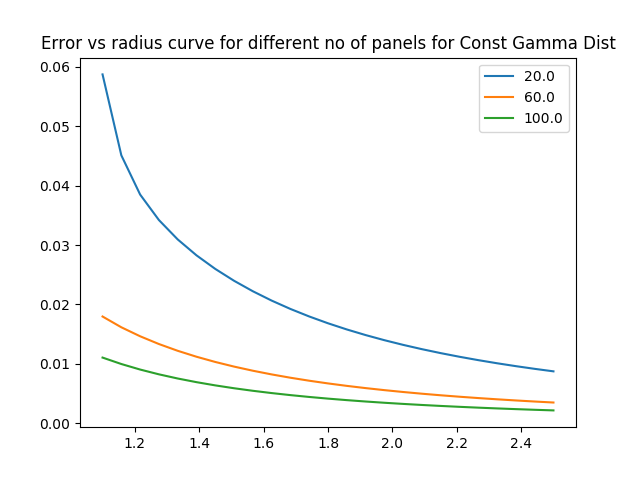
\includegraphics[width = 0.8\textwidth]{q1const_error.png}
		\caption{Error for constant intensity panel method}
		\label{fig:1a}
	\end{figure}
	
	
	
	\indent \textbf{Conclusions:} we can observe that with increase in radius, error is decreasing because
	flow is going close to freestream and close to cylinder there are approximation errors.   .
	As the number of panels is inceased the at any given radius error reduces drastically as the gamma distribution can be better approximated.\\
	
	
	\newpage
	\section{Consider the path of a single point vortex of strength 2 pi placed at a radius 1.5 units from the center of the cylinder of unit radius (without any free-stream). Integrate its path using the RK2 scheme. Also solve the same using the method of images and ensure that the paths are similar. Calculate the error.}
	
	\textbf{Results:}
	
	The exact solution for this problem is
	
	\begin{center}
		$ (u - iv) = \frac{i\Gamma}{2\pi(z - \frac{r^2}{z*})} - \frac{i\Gamma}{2\pi(z)}$
	\end{center}
	The time step for RK2 integrator was 0.05 sec\\
	The vortex sheet was simulated for 3.0 sec\\

	
	\begin{figure}[h]
		\centering
		\begin{subfigure}[h]{.5\textwidth}
			\centering
			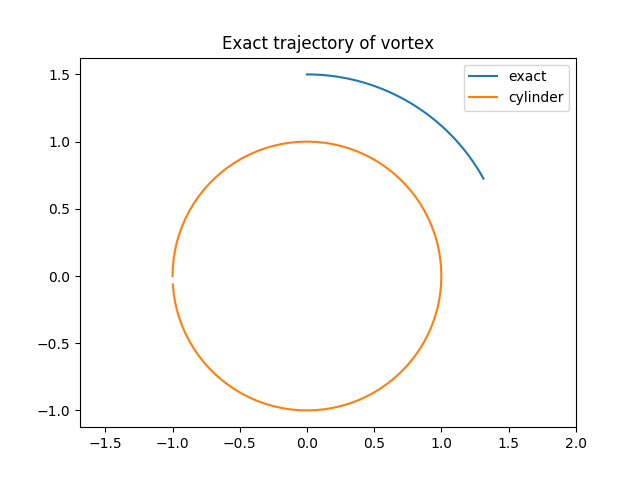
\includegraphics[width=.8\linewidth]{Exact_sol.png}
			\caption{}
			\label{fig:2aa}
		\end{subfigure}%
		\begin{subfigure}[h]{.5\textwidth}
			\centering
			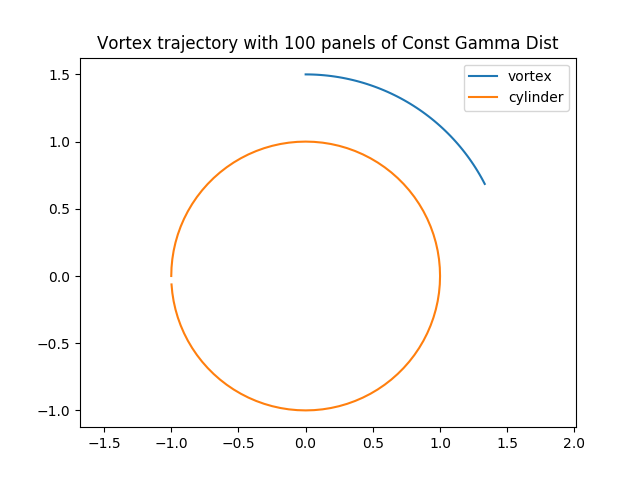
\includegraphics[width=.8\linewidth]{q2const_vort_traj.png}
			\caption{}
			\label{fig:2ab}
		\end{subfigure}
		\caption{Vortex trajectories for const intensity panels}
		
	\end{figure}
	
	\begin{figure}[h]
		\centering
		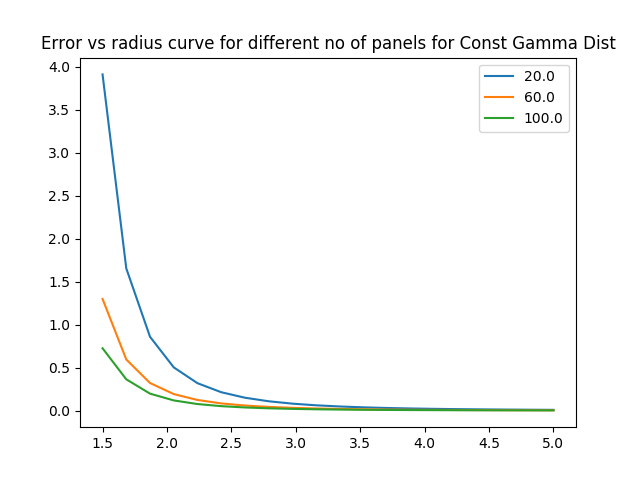
\includegraphics[width = 0.8\textwidth]{q2const_error.png}
		\caption{Error for constant intensity panel method}
		\label{fig:2b}
	\end{figure}
	\newpage 
	\indent\\
	\newpage 
	\indent\\
	\indent \textbf{Conclusions:} Since aprroximated positions of vortex by RK2 are used for calculating the gamma distribution of the panels. The error keeps on building with so panel methods are good for steady state or initial approximation but may not provide accurate results of simulation for large time. 
	
	\newpage
	\section{Do the above for panels with a linear distribution of vorticity on each.}
	
	\textbf{Results:}
	
	The gamma distribution for a single panel is taken as \\
	\begin{center}
		$\gamma _i(x) = \frac{\gamma _{i+1} - \gamma _{i}}{z_{i+1} - z_i} (z - z_{i}) + \gamma _{i}$
	\end{center}
	
	Also velocity induced by a const gamma vortex panel is\\
	\begin{center}$ u - iv = \frac{i}{2\pi}[\frac{\gamma _{i+1} - \gamma _{i}}{z_{i+1} - z_{i}}((z_{i+1} - z_{i}) + (z - z_{i})\log(\frac{z - z_{i+1}}{z - z_{i}})) + \gamma _i\log(\frac{z - z_{i+1}}{z - z_{i}})](\frac{z2 - z1}{{|z1 - z1|}})$\\
		\end{center}
	\indent \indent And the constraint is \\
	\begin{center}
		$\sum_{i = 1}^{n} \gamma _i \frac{(\lambda _i + \lambda _{i+1})}{2} = 0$
	\end{center}
	
	
	\begin{figure}[h]
		\centering
		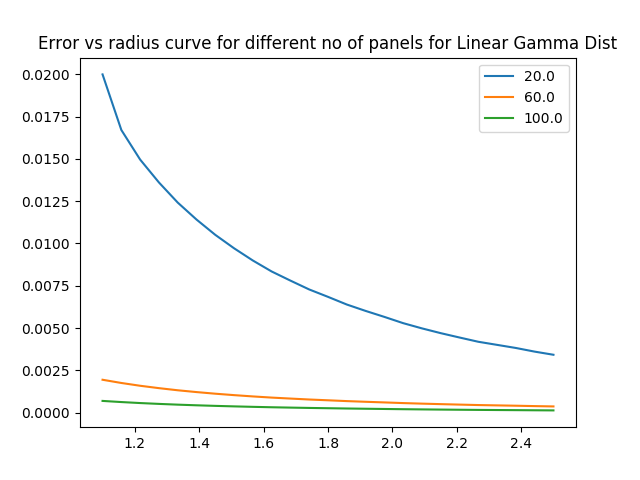
\includegraphics[width = 0.8\textwidth]{q1linear_error.png}
		\caption{Error for linear intensity panel method}
		\label{fig:3a}
	\end{figure}
		\begin{figure}[h]
			\centering
			\begin{subfigure}[h]{.5\textwidth}
				\centering
				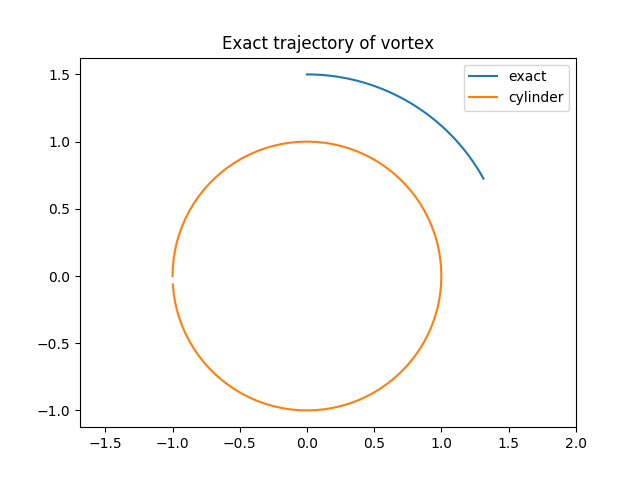
\includegraphics[width=.8\linewidth]{Exact_sol.png}
				\caption{}
				\label{fig:3aa}
			\end{subfigure}%
			\begin{subfigure}[h]{.5\textwidth}
				\centering
				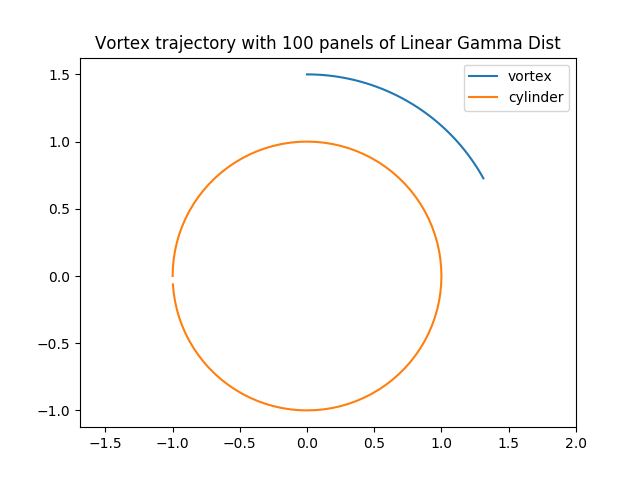
\includegraphics[width=.8\linewidth]{q2lin_vort_traj.png}
				\caption{}
				\label{fig:3ab}
			\end{subfigure}
			\caption{Vortex trajectories for linear gamma panels}
			
		\end{figure}
	\begin{figure}[h]
	\centering
	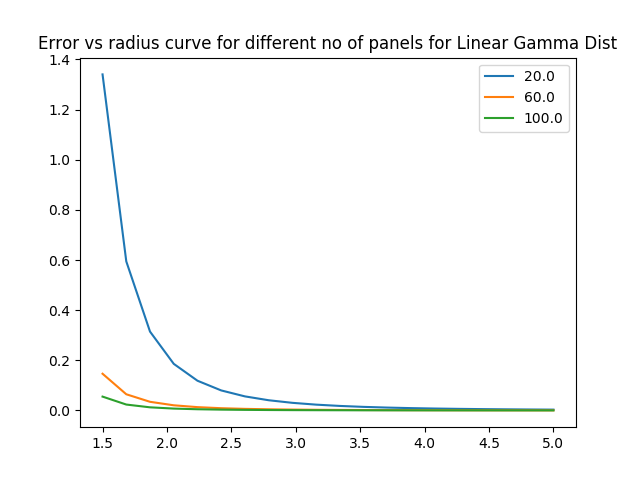
\includegraphics[width = 0.8\textwidth]{q2linear_error.png}
	\caption{Error for linear intensity panel method}
	\label{fig:3b}
	\end{figure}
	\indent 
	\newpage 
	\indent\\
	\newpage
	\indent \textbf{Conclusions:} The trends are similar for Linear intensity vortex panel method. But the error values are significantly lower than Constant intensity vortex panel method.   
	
	
	
	
\end{document}
